
\section{项目成果}

\subsection{实物图片}

\begin{figure}[H]
    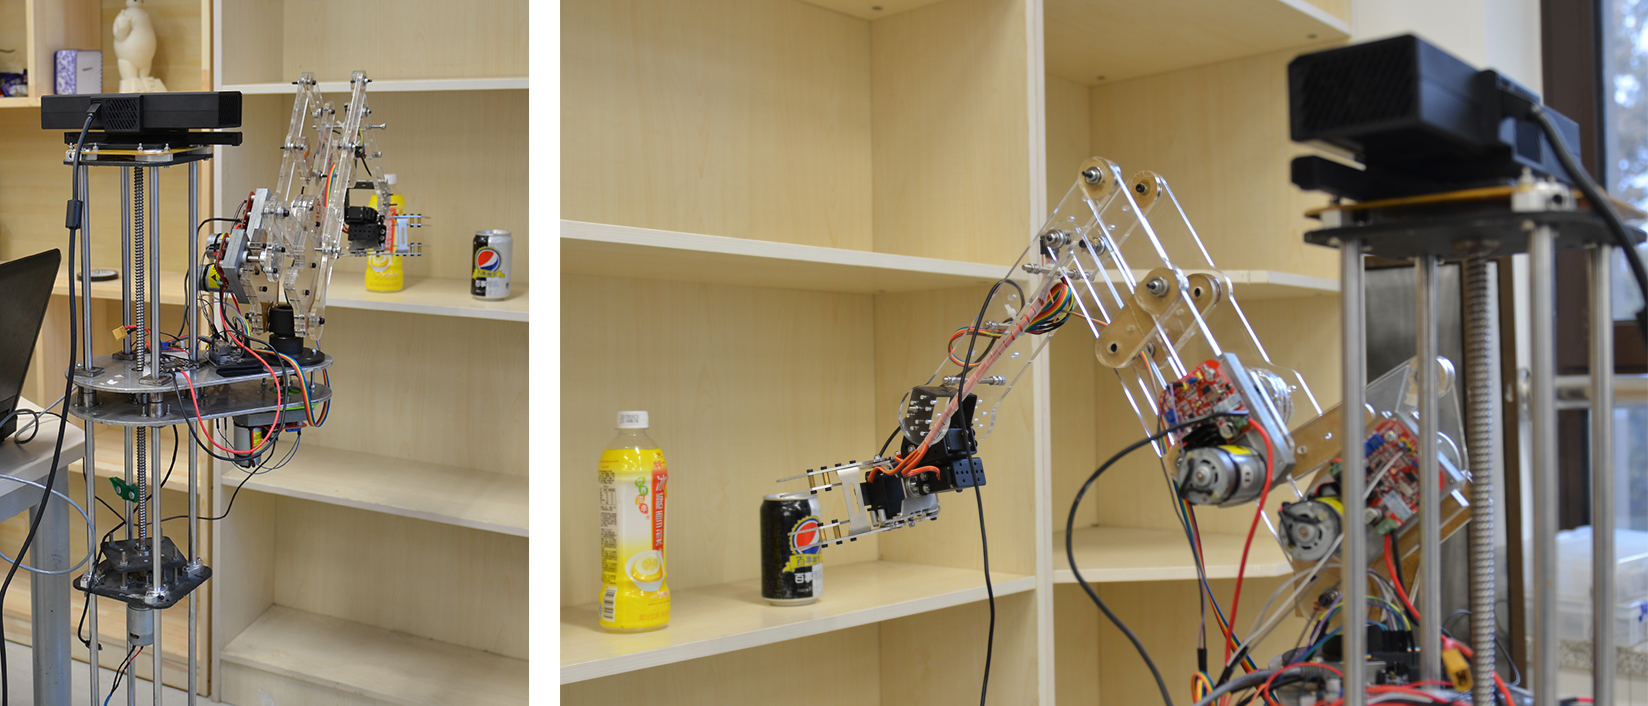
\includegraphics[width = \textwidth]{pictures/1.png}
    \caption{第一版机械臂实物图}
    \label{fig:1}
\end{figure}

\begin{figure}[H]
    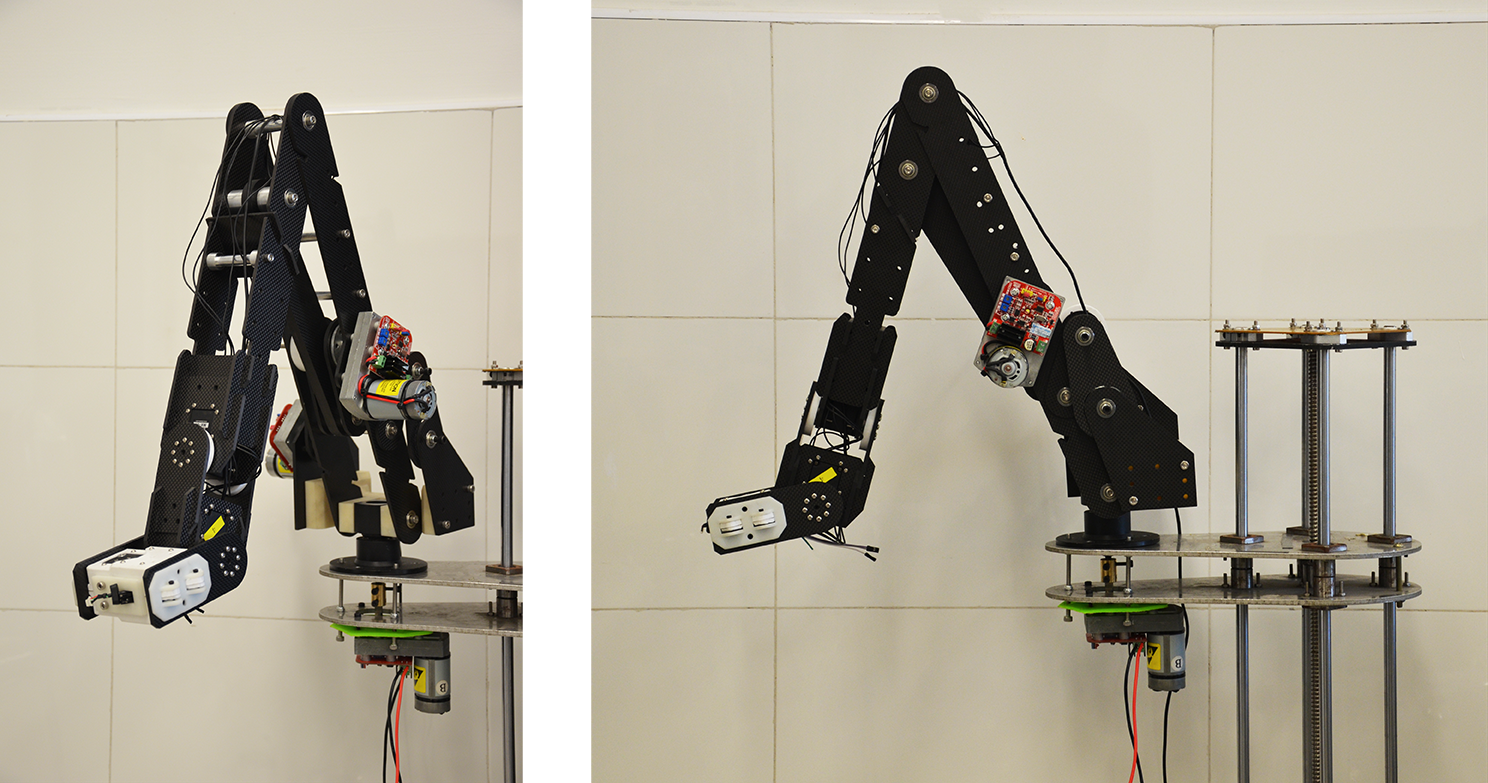
\includegraphics[width = \textwidth]{pictures/2.png}
    \caption{第二版机械臂实物图(仍在制作中)}
    \label{fig:1}
\end{figure}
\subsection{测试结果}

图像处理的测试结果见图\ref{fig:registered},\ref{fig:entropy_block},\ref{fig:downsampled_filled},\ref{fig:color_block},\ref{fig:raw_contour},\ref{fig:after_contour},\ref{fig:final_contour},\ref{fig:lines}所示。

立体视觉获得的点云处理结果如图\ref{fig:initial_pc},\ref{fig:bg},\ref{fig:obj},\ref{fig:clustering},\ref{fig:alp},\ref{fig:baymax}所示。

物体识别的测试结果见图\ref{fig:du1}, \ref{fig:du2}。图\ref{fig:du1}中,左侧窗格显示的sci代表相似度,name代表识别出的物体。

\begin{figure}[H]
    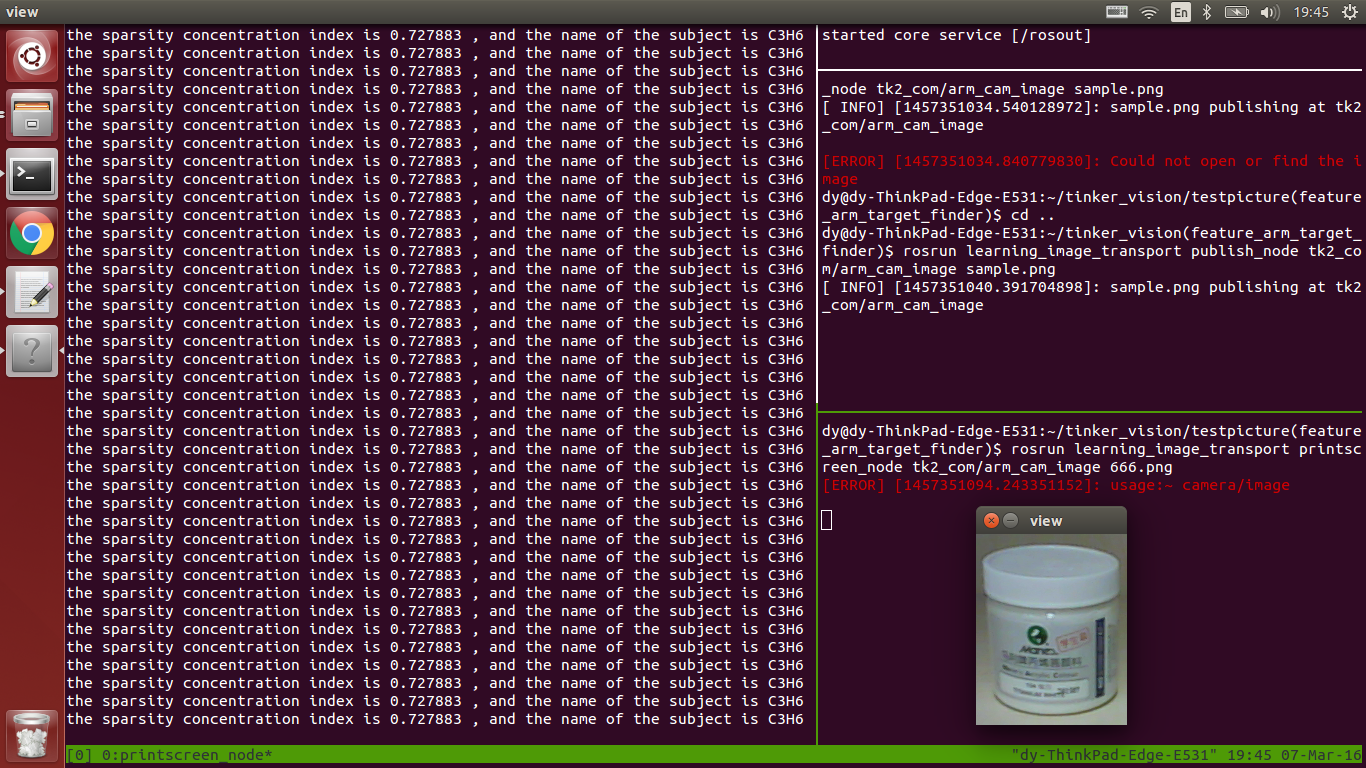
\includegraphics[width = \textwidth]{images/du1.png}
    \caption{物体识别结果}
    \label{fig:du1}
\end{figure}

\begin{figure}[H]
    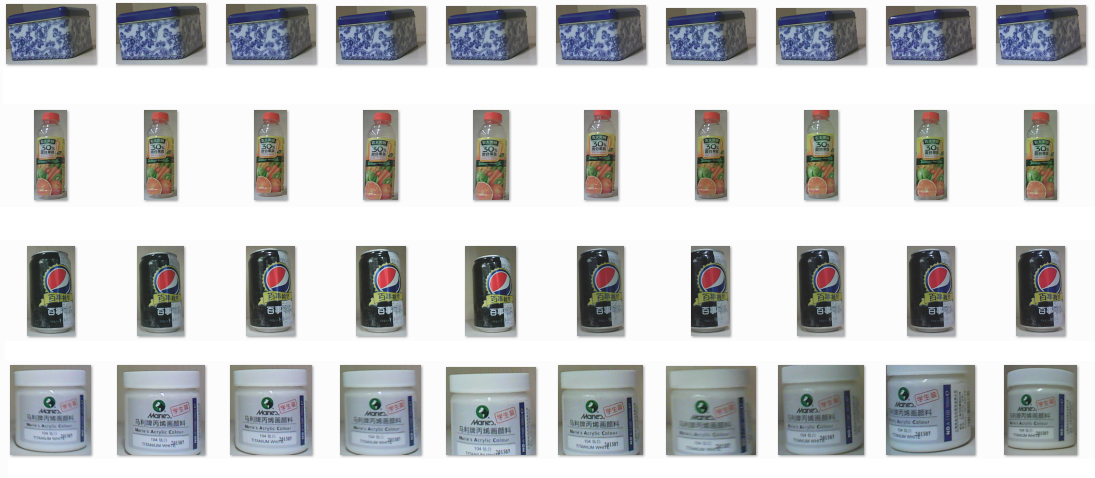
\includegraphics[width = \textwidth]{images/du2.png}
    \caption{物体样本库}
    \label{fig:du2}
\end{figure}

整个系统经测试后能够良好的完成物体定位、识别与抓取任务,具体过程请见视频附件。

\section{发展前景与应用价值}

我们的机械手能够准确的识别物体并抓取,填补了目前家庭机器人市场中缺乏物体移动功能的空缺。在具有了识别并抓取物体的能力后,机械手能够完成许多基本而有必要的家居任务,比如从柜子上取下一个指定的东西送到手边,或者把桌上杂乱的物体排列整齐,在实际的日常生活中也具有较大的应用价值。

\section{总结}

\subsection{项目进展}

目前,我们的项目已经调试通过了所有模块,也在联合调试中测试了整体的性能。\ 我们的机械臂能够准确的识别物体并抓取,最后将其放在指定的地方,达到了预期效果。\ 现在,我们已经根据第一版机械臂的不足设计制造了第二版机械臂,将在之后的一个月内进行调试。项目进度见表\ref{tab:progress}。

\renewcommand\arraystretch{1.2}
\begin{table}[H]
\centering
\begin{tabular}{l|c}
\hline
时间 & 进度 \\ \hline
2015.9-2015.10 & Kinect测试 \\
 & Kinect物品识别算法开发 \\ \hline
2015.11 & 项目立项,进行可行性分析 \\ \hline
2015.12 & 电机选型、购买与测试 \\ \hline
2016.1 & 初版机械臂设计与加工 \\
 & 机械臂控制算法开发 \\
 & 末端摄像头物品识别算法开发 \\ \hline
2016.3 & 第二版机械臂设计与加工 \\
 & 加入移动平台 \\ \hline
\end{tabular}
\caption{项目进度}
\label{tab:progress}
\end{table}

\newpage

\subsection{展望}

我们的系统还有若干方面有改善与提高的空间。\ 我们希望增加机械手的自由度,配合图像算法,使其能够从最合适的方向抓取物体,增加在实际场景中的适应能力;使用如激光雷达来知周围的环境,让我们的机械臂能够更加灵活自主的在房间中移动;语音系统与人脸识别系统,让机械臂能够与人更好的交互。

希望我们的机械臂能走近更多的家庭,帮助人们分担更多的家务,让人们的家居生活更加简单轻松。
